\documentclass[bachelor, och, pract]{SCWorks}
\usepackage[T2A]{fontenc}
\usepackage[utf8]{inputenc}
\usepackage{graphicx}
\usepackage[sort,compress]{cite}
\usepackage{amsmath}
\usepackage{amssymb}
\usepackage{amsthm}
\usepackage{fancyvrb}
\usepackage{longtable}
\usepackage{array}
\usepackage[english,russian]{babel}
\usepackage{minted}
\usepackage{tempora}
\usepackage{titlesec}
\usepackage[colorlinks=false]{hyperref}
\usepackage{xcolor}
\usepackage{hyperref}

\definecolor{linkcolor}{HTML}{799B03} % цвет ссылок
\definecolor{urlcolor}{HTML}{799B03} % цвет гиперссылок

\hypersetup{pdfstartview=FitH,  linkcolor=linkcolor,urlcolor=urlcolor, colorlinks=true}

\hypersetup{ %содержание
colorlinks,
citecolor=black,
filecolor=black,
linkcolor=black,
urlcolor=black
}
\theoremstyle{remark}
\newtheorem{theorem}{Теорема}
\newtheorem{definition}{Определение}
\newtheorem{comment}{Замечание}

\begin{document}
    \hfill \break
    \hfill \break
    \hfill \break
    \hfill \break
    \hfill \break
    \hfill \break
    \hfill \break
    \hfill \break
    \hfill \break
    \hfill \break
    \hfill \break
    \hfill \break
    \begin{center}
        \Huge Лекции по Операционным системам
    \end{center}
    \hfill \break
    \hfill \break
    \hfill \break
    \hfill \break
    \hfill \break
    \hfill \break
    \hfill \break
    \hfill \break
    \hfill \break

    \begin{center} Сверстал: Кузякин Никита Александрович \end{center}
    \begin{center} По лекциям ИТМО \end{center}
    \begin{center}Плейлист с лекциями "--- \href{https://www.youtube.com/watch?v=NctMiqgVRxA&list=PLBWafxh1dFuyGGcWXmR_EngRkoUWvDFJi&index=1}{тут}\end{center}
    \thispagestyle{empty} % выключаем отображение номера для этой страницы
     
    \newpage
    \tableofcontents

    \section{Архитектура компьютерных систем}

    Первоначальными двумя архитектурами компьютерных систем являются Гарвардская и Неймановская архитектуры.

    \begin{figure}[H]
        \begin{center}
            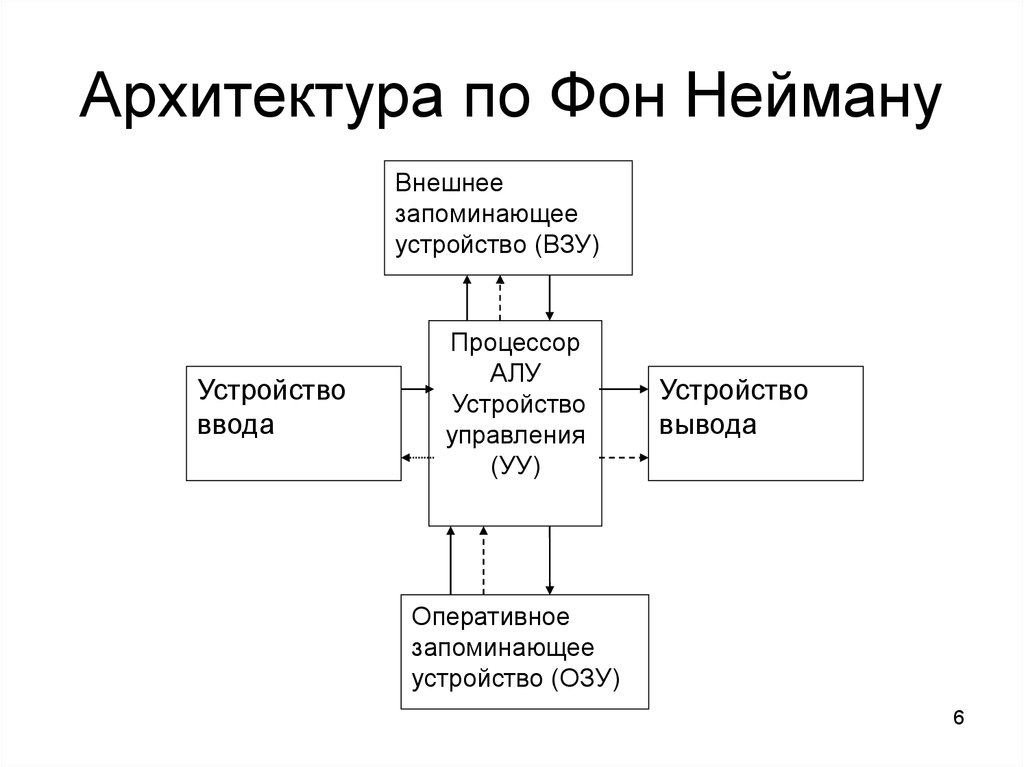
\includegraphics[scale=0.7]{res/Neumann_architecture.png}
        \end{center}
    \end{figure}

    \begin{figure}[H]
        \begin{center}
            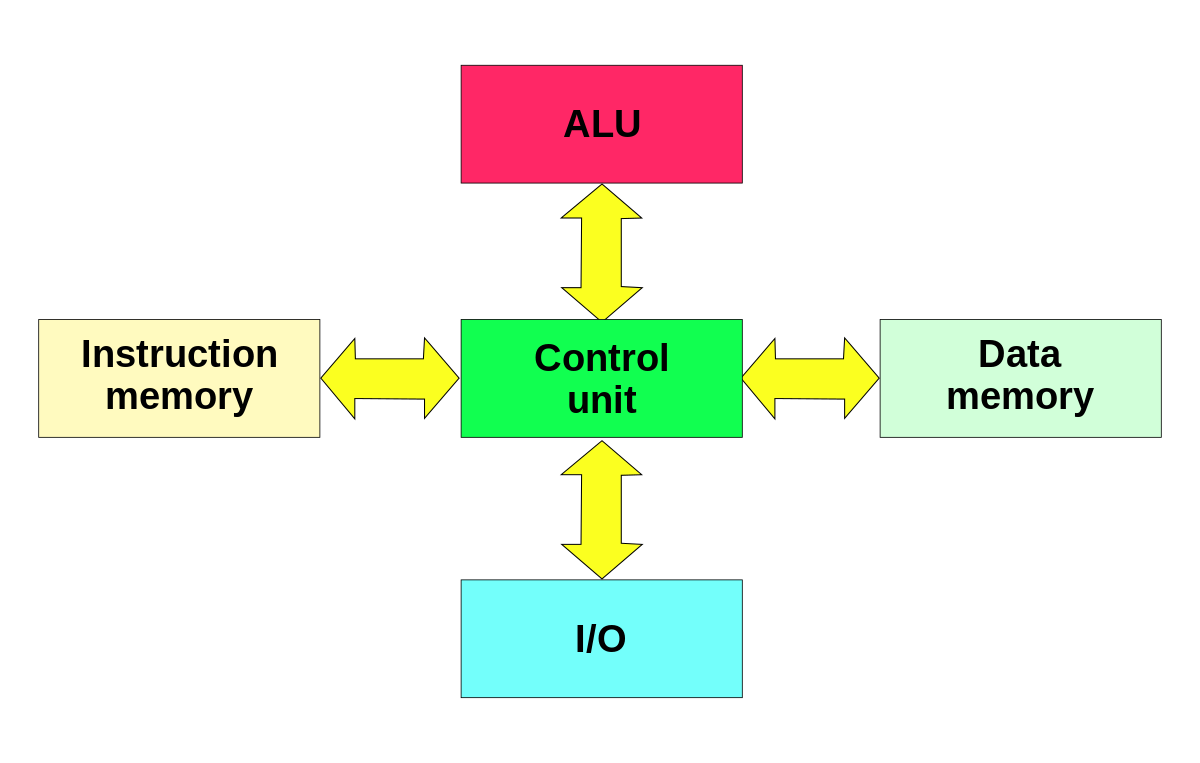
\includegraphics[scale=0.3]{res/Harvard_architecture.png}
            \caption{Гарвардская архитектура ЭВМ}
        \end{center}
    \end{figure}

    Любая вычислительная машины состоит из управляющего устройства (организует вычисления) и арифметико "= логического устройства (производит вычисление арифметических операций), а также различных видов памяти.
    
    В архитектуре фон Неймана предполагается, что есть единое управляющие устройство, память при этом общая (и данная, и программа в одно блоке).

    \textbf{Принципы архитектуры фон Неймана:} 

    \begin{itemize}[label=$\bullet$]
        \item Принцип однородности памяти "--- команды и данные хранятся в одной и той же памяти (внешне неразличимы).
        \item Принцип адресности "--- память состоит из пронумерованных ячеек, процессору доступна любая ячейка.
        \item Принцип программного управления "--- вычисления представлены в виде программы, состоящей из последовательности команд.
        \item Принцип двоичного кодирования "--- вся информация, как данные, так и команды, кодируются двоичными цифрами 0 и 1.
    \end{itemize}

    \hfill \break
    \begin{center}
        \textbf{UMA / NUMA}        
    \end{center}

    В архитектуре U\textbf{UMA} подразумевается, что все устройства являются одноранговыми. Те у любого устройства в системе равные права на доступ к памяти и системные характеристики обращения к ней. 

    \begin{figure}[H]
        \begin{center}
            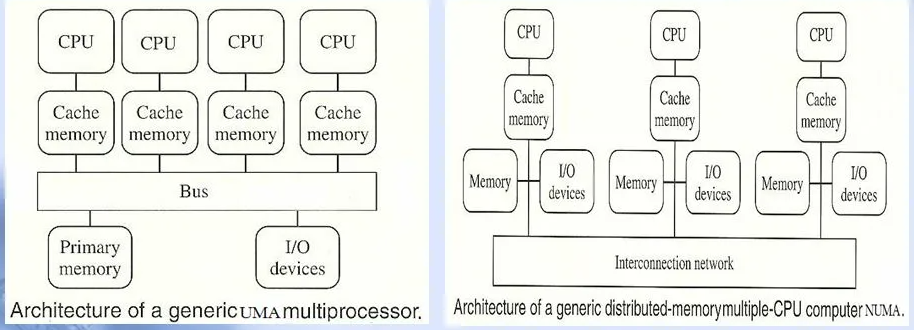
\includegraphics[scale=0.5]{res/UMA-NUMA_architecture.png}
            \caption{Гарвардская архитектура ЭВМ}
        \end{center}
    \end{figure}

    Минусом данной архитектуры является, то что тяжело организовать доступ к памяти для большого числа процессоров.

    В архитектуре \textbf{NUMA} у нас есть память, которая находится ближе к какому-то процессору и память, которая доступна через коммутатор (передает данные через порты). 

    Адресное пространство для данной архитектуры является общим.

    Огромным плюсом является, что можно заменять ее части прямо во время работы, что сильно повышает надежность системы.

    \section{Обзор элементов компьютерных систем}
    
    \subsection{Процессор}
    \begin{figure}[H]
        \begin{center}
            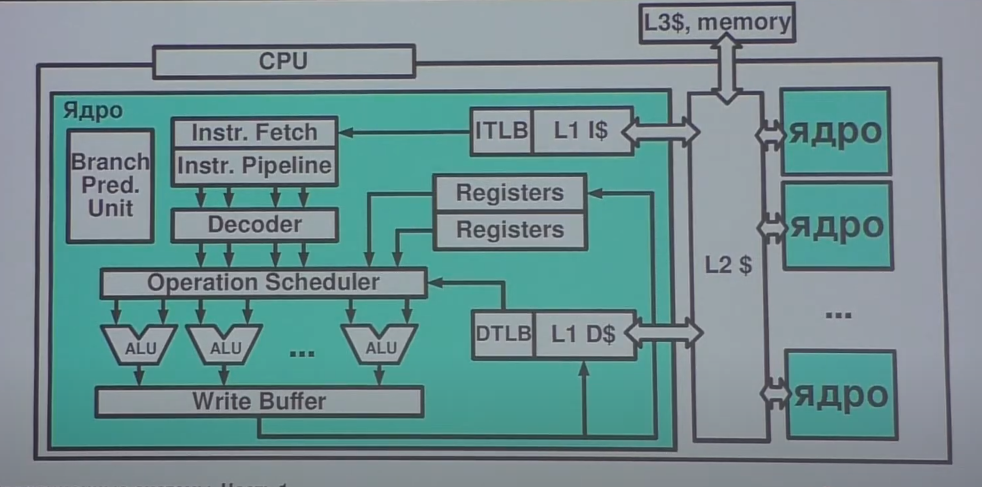
\includegraphics[scale=0.5]{res/processor.png}
        \end{center}
    \end{figure}

    Составляющие: 
    
    \begin{enumerate}
        \item Арифметико-логическое устройство (АЛУ), выполняющее действия над операндами.
        \item Буфер ассоциативной трансляции (TLB) "--- хранит информацию, есть ли такие"=то данные в данном кэше.
        \item Кэш процессора, используемый микропроцессором компьютера для уменьшения среднего времени доступа к компьютерной памяти. Делится на L1 i и L1 d. Один из них хранит набор инструкций для работы с кэшем, другой данные.
        \item Регистры для хранения данных, адресов и служебной информации.
        \item Декодер команд.
        \item Буфер для записи "--- хранит данные, пока буфер не освободится для записи.
        \item Branch Pred. Unit "--- предполагает куда будут записаны данные, по какому адресу (последовательно или с каким"=то отступом).
        \item Instr. Pipeline "--- это метод реализации параллелизма на уровне команд в пределах одного процессора.
    \end{enumerate}

    \hfill \break
    Важно помнить, что процессор выполняет команды последовательно. Пока один компонент выполняет одно действие, другой выполняет другое (они не останавливаются пока одни данные пройдут от начала до конца).

    \begin{definition}
        \textbf{Виртуальная память} "--- это подход к управлению памятью компьютером, который скрывает физическую память (в различных формах, таких как: оперативная память, ПЗУ или жесткие диски) за единым интерфейсом, позволяя создавать программы, которые работают с ними как с единым непрерывным массивом памяти с произвольным доступом.
    \end{definition}

    \begin{figure}[H]
        \begin{center}
            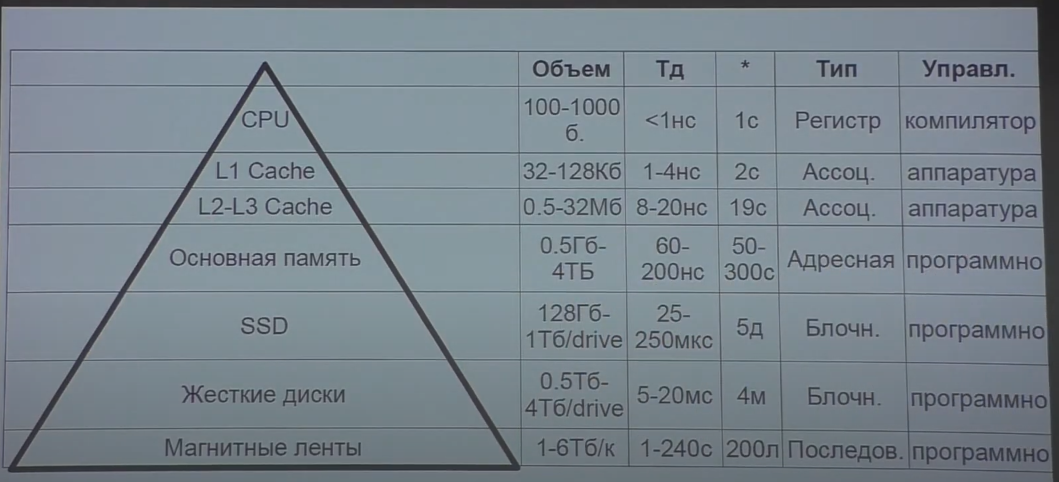
\includegraphics[scale=0.4]{res/memory-pyramid.png}
        \end{center}
    \end{figure}

    Управляется компилятором "--- означает, что именно компилятор определяет, как именно ваша программа будет взаимодействовать с данным блоком памяти, те что в какие регистры запишется и тд. 


    \section{Общие сведения об операционных системах}
    
    \subsection{Функции OS}
    
    \begin{itemize}[label=$\bullet$]
        \item Разработка программ.
        \item Выполнение программ.
        \item Доступ к устройствам ввода / вывода.
        \item Контролируемый доступ к файлам.
        \item Доступ к системе и системным ресурсам.
        \item Обнаружение и обработка ошибок.
        \item Учет пользования и диспетчеризация ресурсов.
        \item Предоставление ключевых интерфейсов (ISA "--- набор команд, ABI "--- бинарный интерфейс приложения, API "--- интерфейс прикладных программ).
    \end{itemize}
    
    \subsection{Оператор ЭВМ}
    Что должен делать оператор?
    \begin{enumerate}
        \item получить программу с данными от программиста.
        \item подготовить программу к загрузке.
        \item загрузить программу и компилятор.
        \item запустить программу на вычисление.
        \item распечатку с результатом передать программисту.
    \end{enumerate}

    Минусами оператора ЭВМ является: наличие расписания машинного времени и долгое время подготовки к работе.

    \subsection{Пакетная обработка}
    В следствие минусов оператора ЭВМ появилась пакетная обработка.

    Появился первый Системный монитор, который включал в себя: обработчик прерываний, драйверы устройств, планировщик заданий, интерпретатор командного языка и было отведено пространство под пользовательские программы и данные.


    \subsection{Многозадачность}

    Одним из главных минусов первых ЭВМ было то, что вовремя вывода, ввода или работы других устройств процессор простаивал. В следствие этого появилась концепция многозадачности.

    \begin{figure}[H]
        \begin{center}
            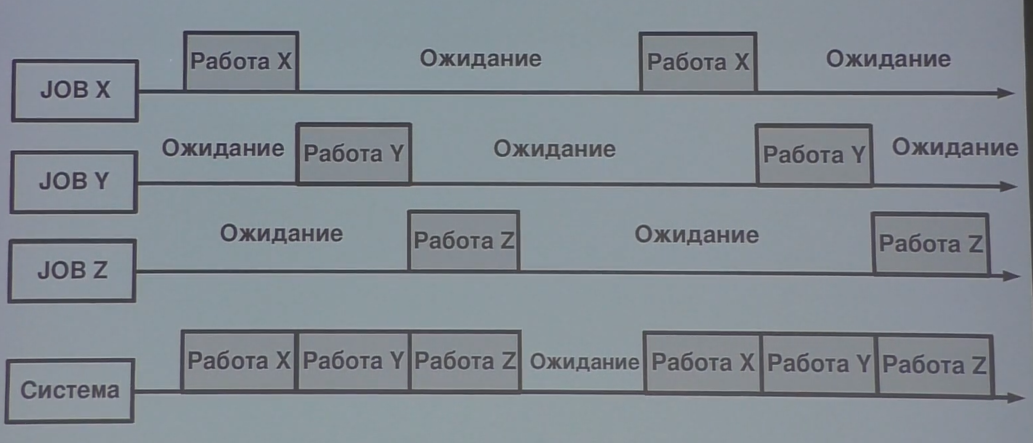
\includegraphics[scale=0.4]{res/multitasking.png}
            \caption{Схема многозадачности первых ЭВМ}
        \end{center}
    \end{figure}
    
    \subsection{Разделение времени}
    
    Следующим нововведением в ЭВМ стало исключение оператора и добавление пользователей. Каждому пользователю выдавалось часть времени процессора с использованием квантового времени. В следствие этого появились проблемы разделения ресурсов и защита одних программ от других.

    \section{Основные задачи OS}

    \subsection{Управление процессами}

    \begin{definition}
        \textbf{Процесс} (с точки зрения обывателя) "--- экземпляр программы во время ее исполнения.
    \end{definition}
    
    \begin{definition}
        \textbf{Процесс} (с точки зрения OS) "--- единица потребления ресурсов OS, в которой существует последовательность действий, текущее состояние и набор связанных ресурсов.
    \end{definition}
    
    \begin{figure}[H]
        \begin{center}
            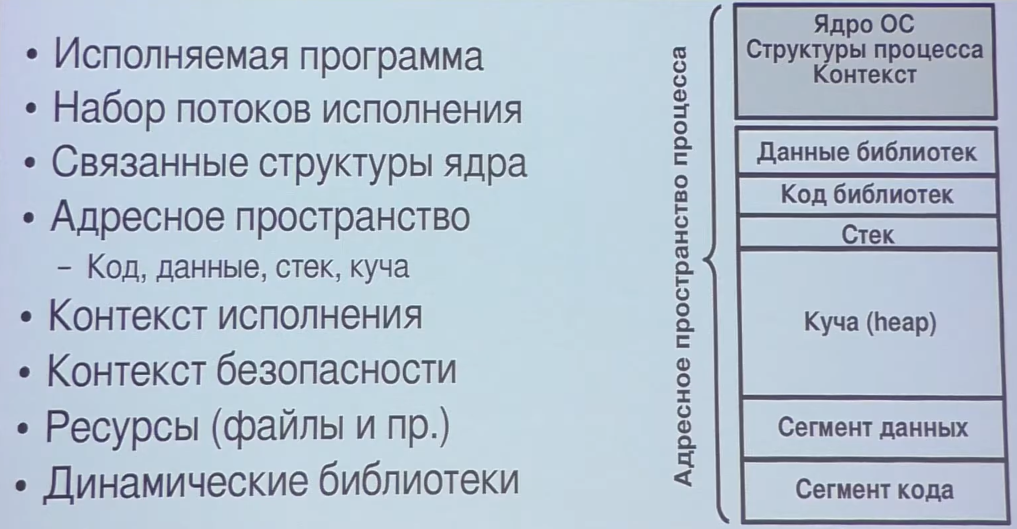
\includegraphics[scale=0.4]{res/process-structure.png}
            \caption{Структура процесса}
        \end{center}
    \end{figure}

    Для того, чтобы создать процесс, необходимо создать все части адресного пространства представленного на рисунке 4.

    Процесс создается не так быстро, поэтому для вычислений на процессоре можно просто создать поток (по сути он будет представлять набор регистров) и с помощью него провести вычисления. Это все и является контекстом.

    Когда создается процесс, ядро OS должно построить для ресурсов, которое он будет потреблять систему (описание ресурсов) (в линуксе task structure). 

    Проблемы современных процессов:

    \begin{itemize}[label=$\bullet$]
        \item Защита памяти процессов "--- недетерминированное поведение процесса, к примеру обращение не к своей памяти, может нарушить другие процессы.
        \item Взаимные блокировки "--- есть два процесса, один из них захватил один ресурс, другой другой, и они пытаются также добавить к себе захваченный другим процессом ресурс. (deadlock, livelock, starvation)
        \item Проблема синхронизации "--- тк у нас может быть несколько процессов, а адресное пространство для них одно.
        \item Взаимное исключение доступа ресурсов.
    \end{itemize}

    \subsection{Виртуальная память}
    Для решения проблемы с единым адресным пространством была придумана виртуальная память.

    Управление памятью: 
    \begin{itemize}[label=$\bullet$]
        \item Изоляция процессов.
        \item Управление выделением и освобождением памяти (аллокаторы и мепинг памяти).
        \item Поддержка модулей (модульности) "--- динамическая загрузка и выгрузка модулей.
        \item Защита и контроль доступа "--- права на сегменты памяти.
        \item Долговременное хранение "--- запись информации на диск.
        \item Страничный обмен. 
    \end{itemize}

    \begin{definition}
        \textbf{Виртуальная память} "--- отдельное виртуальное адресное пространство для каждого процесса и ядра.
    \end{definition}

    Также виртуальная память подразумевает, что некоторые страницы нельзя выгружать из памяти, к примеру если они используются в большом количестве процессов.
    
    \subsection{Безопасность}
    Также важный аспект OS это то, на сколько она безопасна, на сколько она обеспечивает безопасность данных.

    Самым важным аспектом безопасности является протокол работы с информацией.

    Что должна обеспечивать OS:

    \begin{enumerate}
        \item Безопасность доступа к системе "--- защита от несанкционированного доступа.
        \item Конфиденциальность "--- невозможность неавторизованного доступа к данным.
        \item Целостность данных "--- защита данных от неавторизованного и нецелостного изменения.
        \item Аутентификация и авторизация.
    \end{enumerate}

    \subsection{Диспетчеризация и планирование ресурсов}

    Что важно учесть при планирование ресурсов (с точки зрения OS):

    \begin{itemize}[label=$\bullet$]
        \item Равноправие "--- пользователи, процессы и тд должны получать ресурсы равноправно. (Интересный факт: в UNIX приоритет процесса развернутого окна на 15 пунктов выше других).
        \item Дифференциация отклика "--- в некоторых задачах нужно понизить время отклика, к примеру в задачах выполняющихся в реальном времени.
        \item Общесистемная эффективность.
        \item Планировщик процессов, дисков и тд.
    \end{itemize}


    \section{Современные архитектурные концепции OS}

    \subsection{Архитектура ядер}

    \begin{figure}[H]
        \begin{center}
            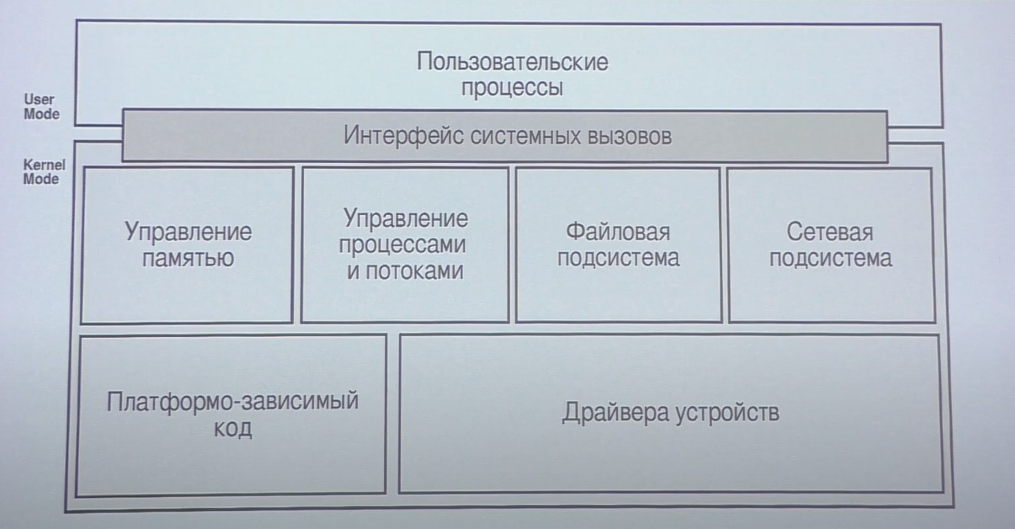
\includegraphics[scale=0.4]{res/OS-kernel-diagram.png}
            \caption{Схема ядра OS}
        \end{center}
    \end{figure}

    Управление памятью, процессами и потоками, файловая подсистема и сетевая подсистема работают на основе драйверов и платформо "= зависимого кода.

    \begin{figure}[H]
        \begin{center}
            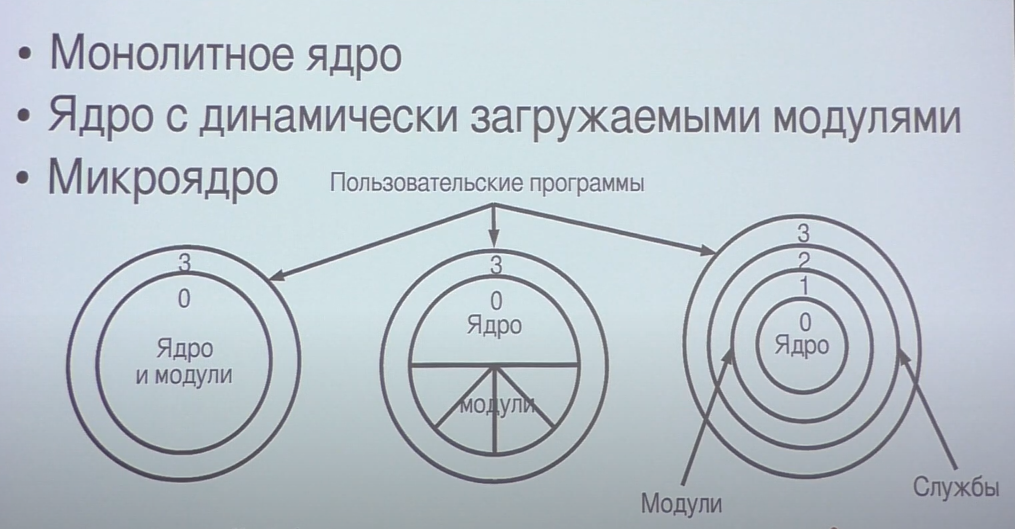
\includegraphics[scale=0.4]{res/kernel-architectures.png}
            \caption{Виды архитектур ядер OS}
        \end{center}
    \end{figure}

    Монолитное ядро "--- подразумевает, что для изменение чего"=то в ядре придется перекомпилировать OS. Подходит для систем где набор устройств определен и не будет изменяться. 0 уровень "--- ядро и встроенные в него модули, 3 уровень "--- пользовательские программы. 1 и 2 не используются.

    Ядро с динамически загружаемыми модулями имеет возможность загрузить модули во время выполнения операционной системы.
    
    Микроядро "--- концепция, в которой само ядро занимается базовыми задачами: диспетчеризация процессов и выделение памяти. 1 и 2 уровни занимают остальные задачи, реализованные в виде сервисов. Пользовательские приложения работают на 3 уровне. Из"=за частого переключения контекстов это работает очень медленно. 

    \subsection{Многопоточность}
    Из"=за сложности создания процесса была придумана концепция реализации внутри процесса потоков. Tread "--- нить / поток.

    Библиотека порождающая потоки на UNIX системах Posix Treads.
    
    Существует множество концепций реализации потоков, они будут рассмотрены в следующих параграфах.

    \subsection{SMP и ASMP}
    
    \textbf{Symmetric multiprocessing} "--- процессы равны, процесс выполняется на нескольких процессорах одновременно. Это дает следующие плюсы: простота разработки и производительность, более высокая надежность (при отказе выполнить процесс, его могут выполнить другие), масштабируемость приложений, динамическое добавление ресурсов процессора. 

    \textbf{Asymmetric multiprocessing} "--- в системе с асимметричной многопроцессорностью не все процессоры играют одинаковую роль. Например, система может использовать (либо на аппаратном, либо на уровне операционной системы) только один процессор для выполнения кода операционной системы, или поручать только одному процессору выполнение операций ввода-вывода. В других AMP-системах все процессоры могут выполнять код операционной системы и операции ввода-вывода, так что с этой стороны они ведут себя как симметричная многопроцессорная система, но определенная периферийная аппаратура может быть подсоединена только к одному процессору, так что со стороны работы с этой аппаратурой система предстаёт асимметричной. Более дешевая альтернатива в системах, которые поддерживали SMP.
 
    \textbf{Многопоточность $!=$ Многопроцессорность}

    \subsection{Виртуализация}

    \textbf{Виртуальные машины (интерпретаторы)} "--- по сути программы, которые работают под выполнением другой программы. Как примеры: JS в браузере, python, JAVA VM. Это позволяет поднять уровень абстракции.

    \begin{definition}
        \textbf{Интерпрета́ция} — построчный анализ, обработка и выполнение исходного кода программы или запроса, в отличие от компиляции, где весь текст программы, перед запуском анализируется и транслируется в машинный или байт-код без её выполнения.
    \end{definition}

    \textbf{Контейнеры приложений} "--- позволяет писать приложения один раз и запускать их где угодно. Разработчики могут создавать и развертывать приложения быстрее и безопаснее, чем при традиционном подходе к написанию кода — когда он разрабатывается в определенной вычислительной среде, а его перенос в новое место, например из тестовой среды в продуктивную, часто приводит к ошибкам выполнения кода.

    \begin{definition}
        \textbf{Контейнер приложения} "--- экземпляр исполняемого программного обеспечения (ПО), который объединяет двоичный код приложения вместе со всеми связанными файлами конфигурации, библиотеками, зависимостями и средой выполнения.
    \end{definition}

    Смысл и главное преимущество технологии в том, что контейнер абстрагирует приложение от операционной системы хоста, то есть остается автономным, благодаря чему становится легко переносимым — способным работать на любой платформе.

    Примеры: Docker, Solaris containers, Linux containers. 

    \textbf{Аппаратурная виртуализация} "--- виртуализация с поддержкой специальной процессорной архитектуры. В отличие от программной виртуализации с помощью данной техники возможно использование изолированных "гостевых" операционных систем.

    Примеры: Virtual BOX, KVM.


    \textbf{Облачные технологии} "--- по сути облачная виртуализация, главным плюсом является, что в случае сбоя одной физической системы, данные иммигрируют на другую систему и продолжат выполняться. Данные технологии построены на базе аппаратурной виртуализации.



    \section{Полезные утилиты}

    Google Test Framework "--- \href{https://google.github.io/googletest/primer.html}{https://google.github.io/googletest/primer.html}

\end{document}